\section{Durchführung}
\label{sec:Durchführung}
In diesem Versuch wird ein Acrylblock und ein Brustmodell mittels Ultraschall untersucht. Es genügt aber nicht die Ultraschallsonde auf das zu untersuchende Material zu halten, da sich dann
zwischen der Sonde und dem Material eine Luftschicht befindet. Diese überträgt den Ultraschall nicht genügend an die \textit{Receiver}-Sonde. Dadurch gelingt die Messung nicht. Um dies zu vermeiden
wird eine Anpassungschicht auf das Material aufgetragen. Für den Acrylblock wird destilliertes Wasser verwendet. Diese Wasserschicht nimmt ebenfalls einen Einfluss auf die Messung. Daher werden
zunächst im Rahmen der Vorbereitungsaufgaben einige Materialkonstanten bestimmt.
\subsection{Vorbereitungsaufgaben}
\label{subsec:VBA}
(Ultra-)Schall ist eine Welle, welche sich durch Dichteschwankungen in einem Medium ausbreitet. Da Dichteschwankungen von der Dichte des Ausbreitungsmediums abhängen ist die Schallgeschwindigkeit
eine  Materialkonstante. Für den folgenden Versuch sind drei Schallgeschwindigkeiten relevant. Destilliertes Wasser hat bei $\qty{20}{\celsius}$ eine Schallgeschwindigkeit von $\qty{1483}{\metre\per\second}$.
Die Schallgeschwindigkeit im Acrylblock liegt bei $\qty{2730}{\metre\per\second}$ und die von Luft bei $\qty{20}{\celsius}$ lautet $\qty{344}{\metre\per\second}$.
Es sind in diesem Versuch 2 Messsonden vorhanden. Eine davon sendet Ultraschall mit eine Frequenz von $\qty{1}{\mega\hertz}$ und die andere mit $\qty{2}{\mega\hertz}$. Nun kann mittels Formel
\eqref{eqn:lambda} die Wellenlänge und Periodendauer in Acryl bestimmt werden. Dazu wird die zuvor erwähnte Schallgeschwindigkeit
verwendet. Mit einer Frequenz von $\qty{1}{\mega\hertz}$ ergibt sich dann eine Wellenlänge von $\qty{2.73}{\milli\metre}$ und eine Periodendauer von $\qty{1}{\micro\second}$. Bei $\qty{1}{\mega\hertz}$
liegt die Wellenlänge bei $\qty{1.365}{\milli\metre}$ und die Periodendauer bei $\qty{0.5}{\micro\second}$.
\subsection{Versuchsdurchführung}
\label{subsec:Versuchsdurchführung}
Zur Untersuchung mit Ultraschall wird ein Ultraschallechoskop und Ultraschallsonden verschiedener Frequenzen benötigt. Außerdem wird ein Acrylblock, welcher in \autoref{fig:acrylskizze} skiziert wird, und destilliertes Wasser benötigt. 
Das Ultraschallechoskop wird im Impuls-Echo-Verfahren verwendet. Die Sendefrequenz wird in einem Bereich von $\qty{0}{\decibel}$ bis $\qty{30}{\decibel}$ eingestellt. Die 
Empfängerfrequenz in einem Bereich von $\qty{0}{\decibel}$ bis $\qty{35}{\decibel}$. Das Ultraschallechoskop wird mit einer Rechner verbunden und die Informationen werden dann 
über das Programm \textit{A-Scan} dargestellt. 

\begin{figure}
    \centering
	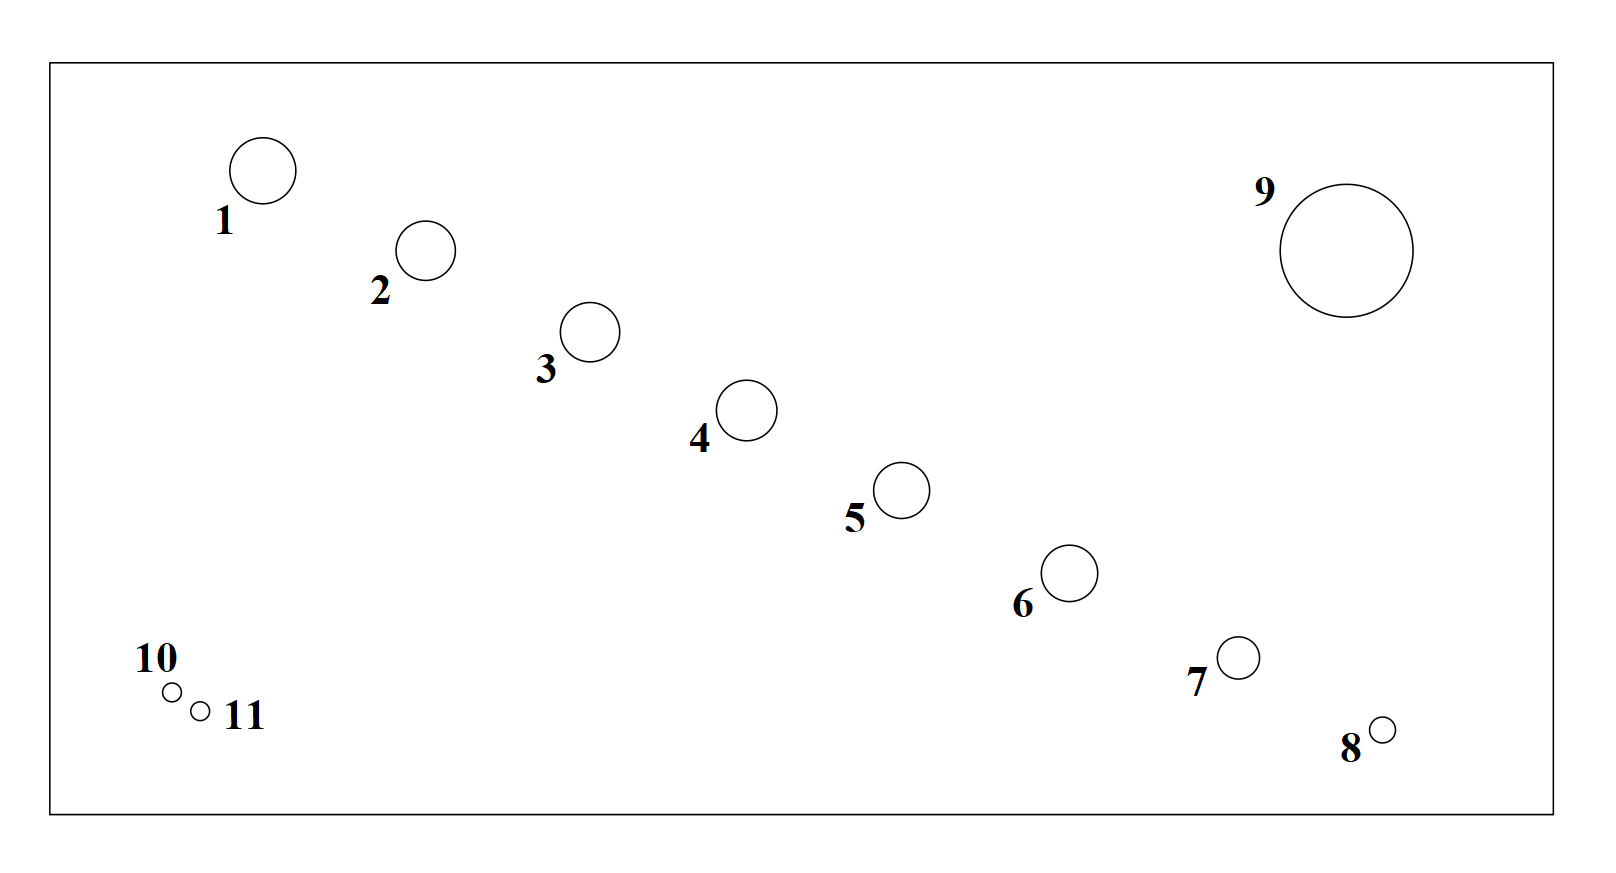
\includegraphics[width=\textwidth]{content/Acrylblock.png}
    \caption{Dies ist eine Skizze des verwendeten Acrylblocks mit den nummerierten Fehlstellen. \cite{vUS2}.}
    \label{fig:acrylskizze}
\end{figure}

Zuerst wird mit der händischen Vermessung des Acrylblocks begonnen. Dabei werden sowohl die Gesamtmaße des Blocks wie auch die einzelnen Positionen und Größen der zu 
Untersuchenden Störstellen bestimmt. Nun wird das Ultraschallechoskop in Betrieb genommen und das Programm \textit{A-Scan} gestartet. Dann wird eine ausreichendgroße Menge destilliertes
Wasser auf den Acrylblock aufgetragen. Es werden jetzt die Laufzeiten für sieben Löcher in dem Acrylblock bestimmt und notiert. Hierzu ist es nicht relevant welche Sonde verwendet wird.
Aus diesen Werten wird dann in \autoref{sec:Auswertung} die Laufzeitgeschwindigkeit und die Dicke der Anpassungschicht bestimmt. Als nächstes wird die Lage aller Löcher im Acrylblock
bestimmt. Nun wird die $\qty{2}{\mega\hertz}$ Sonde verwendet. Die Löcher werden nur von einer Seite des Acrylblocks mit dieser Sonde untersucht. Auch hier wird das Ultraschallechoskop 
im Impuls-Echo-Verfahren verwendet. 
Darauf hin wird der Block auch von der gegenüberliegenden Seite untersucht. Die Einstellungen und das Messverfahren sind indentisch zu dem vorherigen. Daraus kann die genaue
Position und die Größe der Fehlstellen im Acrylblock bestimmt werden.

In dem Acrylblock befinden sich zwei Störstellen, welche unmittelbar nebeneinander liegen. Anhand dieser soll nun das Auflösungsvermögen der Sonden untersucht werden. Zuerst wird 
ein A-Scan dieser Stelle mittels der $\qty{1}{\mega\hertz}$ Sonde angefertigt. Dies wird für die $\qty{2}{\mega\hertz}$ Sonde wiederholt. Die jeweiligen Peaks werden als Graphiken
exportiert.

Zuletzt wird nun ein B-Scan des Acrylblocks angefertigt. Dazu wird die $\qty{2}{\mega\hertz}$ Sonde verwendet. Sobald das Programm für den B-Scan läuft, fährt man mit der Ultraschallsonde
langsam, mit konstanter Geschwindigkeit, in einer geraden Linie über den Acrylblock. Dies wird auf beiden Seiten des Acrylblocks durchgeführt. Der jeweils erstellte B-Scan wird gespeichert.
Mittels der beiden Bilder werden dann die Abmessungen der Störstellen berechnet. 

Nun wird ein neues Material untersucht. Es wird ein Brustmodell untersucht, welches eingebaute Störstellen besitzt. Dieses Modell wird in \autoref{fig:brust} dargestellt. Die Fehlstellen modellieren Tumore. Zu Beginn wird die ungefähre Lage der 
Tumore händisch ertastet. Dann werden die Einstellungen des Ultraschallechoskops angepasst. Dabei wird getestet welche Einstellungen und welche Sonde die klarsten Ergebnisse liefern.
Nun wird mit den ermittelten Einstellungen ein B-Scan durchgeführt. Dazu wird eine Ultraschallflüssigkeit als Kontaktmittel verwendet. Der Scan findet erneut entlang einer geraden 
Linie statt. Es werden solange Scans angefertigt bis die Art, Größe und Lage des Tumors bestimmt werden kann.

\begin{figure}
    \centering
	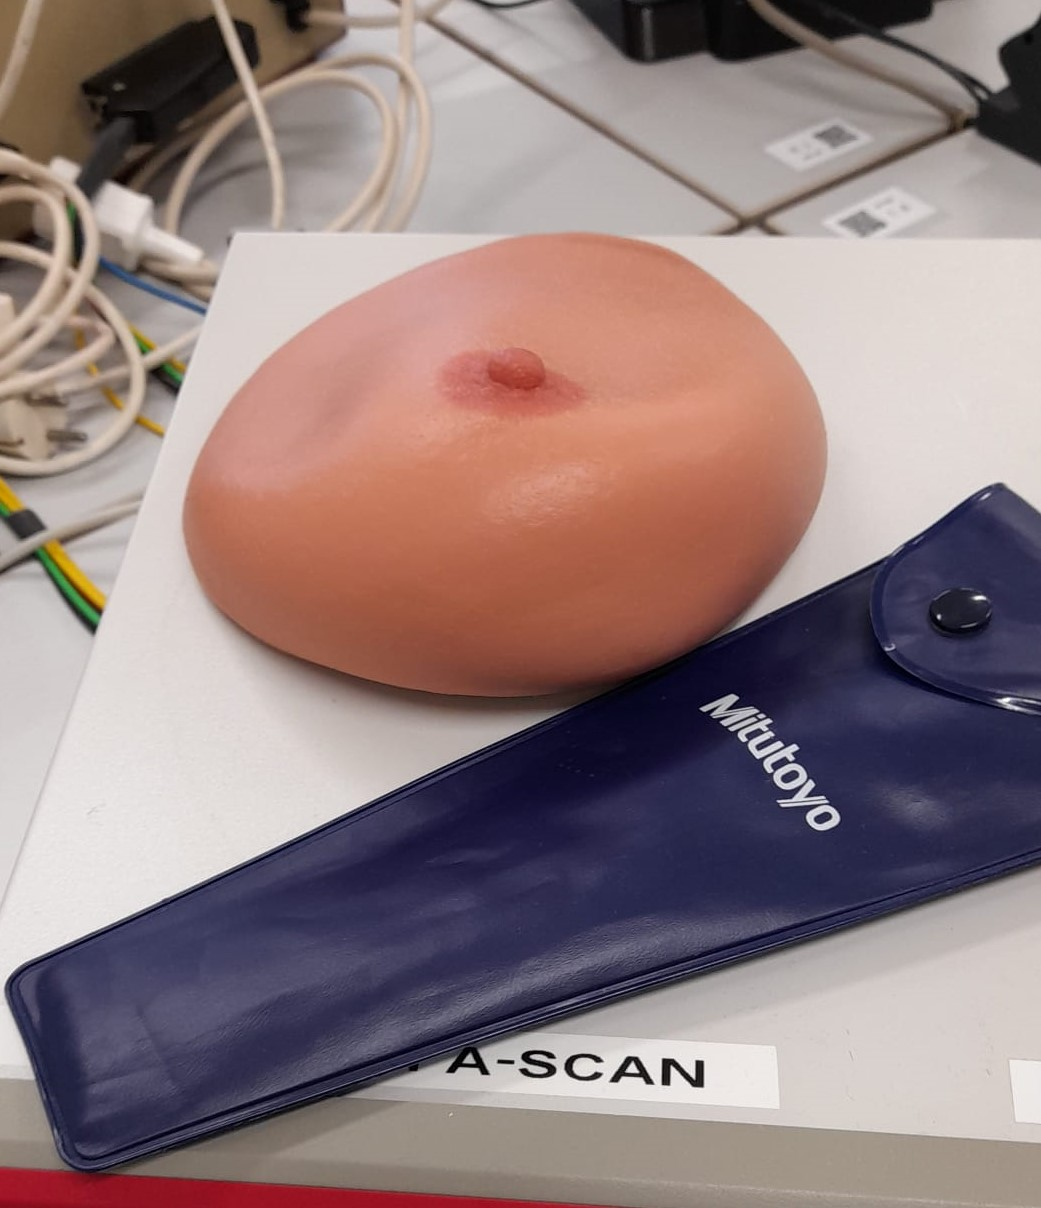
\includegraphics[width=0.5\textwidth]{content/Titte1.jpg}
    \caption{Dies ist ein Bild des verwendeten Brustmodells.}
    \label{fig:brust}
\end{figure}
